\documentclass[tikz,border=4pt]{standalone}
% Estilo común de los diagramas de bloques (se usa con \input en cada standalone)
\usepackage[defaultsans,scale=0.92]{lato}
\usepackage{libertinust1math}
\usepackage{xcolor,amsmath}
\usepackage{tikz}
\usetikzlibrary{positioning,arrows.meta,calc,shapes.geometric}
\usepackage{../../notacion}
\definecolor{ctrlazul}{HTML}{1E5AA8}\definecolor{ctrlnoche}{HTML}{14213D}
\definecolor{ctrlcoral}{HTML}{D1495B}\definecolor{ctrlverde}{HTML}{2A9D8F}
\definecolor{ctrlambar}{HTML}{E09F3E}\definecolor{ctrlgris}{HTML}{5C677D}
\definecolor{ctrlvioleta}{HTML}{6C4AB6}\definecolor{ctrlteal}{HTML}{0F7173}
\tikzset{
  >={Stealth[length=2.4mm]}, every node/.style={font=\small},
  bloque/.style={draw=ctrlnoche,fill=ctrlazul!7,thick,rounded corners=1.5pt,minimum height=9mm,minimum width=13mm,inner sep=4pt},
  suma/.style={draw=ctrlnoche,thick,circle,inner sep=0pt,minimum size=6mm},
  senal/.style={->,thick,draw=ctrlnoche},
  rot/.style={font=\footnotesize,text=ctrlgris},
}

\begin{document}
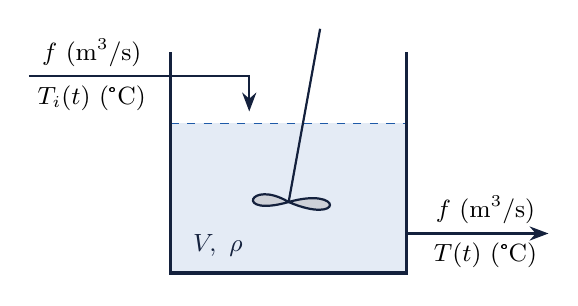
\begin{tikzpicture}[font=\small]
  \fill[ctrlazul!12] (0,0) rectangle (3,1.9);
  \draw[ctrlazul,dashed] (0,1.9)--(3,1.9);
  \draw[very thick,ctrlnoche] (0,2.8)--(0,0)--(3,0)--(3,2.8);
  % agitador
  \draw[thick,ctrlnoche] (1.9,3.1)--(1.5,0.9);
  \draw[thick,ctrlnoche,fill=ctrlgris!30] (1.5,0.9) .. controls (1.0,1.2) and (0.8,0.7) .. (1.5,0.9) .. controls (2.2,1.1) and (2.2,0.6) .. (1.5,0.9);
  % entrada
  \draw[senal] (-1.8,2.5)--(1.0,2.5)--(1.0,2.05);
  \node[above,align=left] at (-1.0,2.5) {$f$ (m$^3$/s)}; \node[below] at (-1.0,2.5) {$T_i(t)$ (°C)};
  % salida
  \draw[senal] (3,0.5)--(4.8,0.5);
  \node[above] at (4.0,0.5) {$f$ (m$^3$/s)}; \node[below] at (4.0,0.5) {$T(t)$ (°C)};
  \node[ctrlnoche] at (0.6,0.35) {$V,\ \rho$};
\end{tikzpicture}
\end{document}
